\begin{figure}[htbp]
\section*{ KDM6B}
\centering
\begin{subfigure}[b]{0.95\textwidth}
\centering
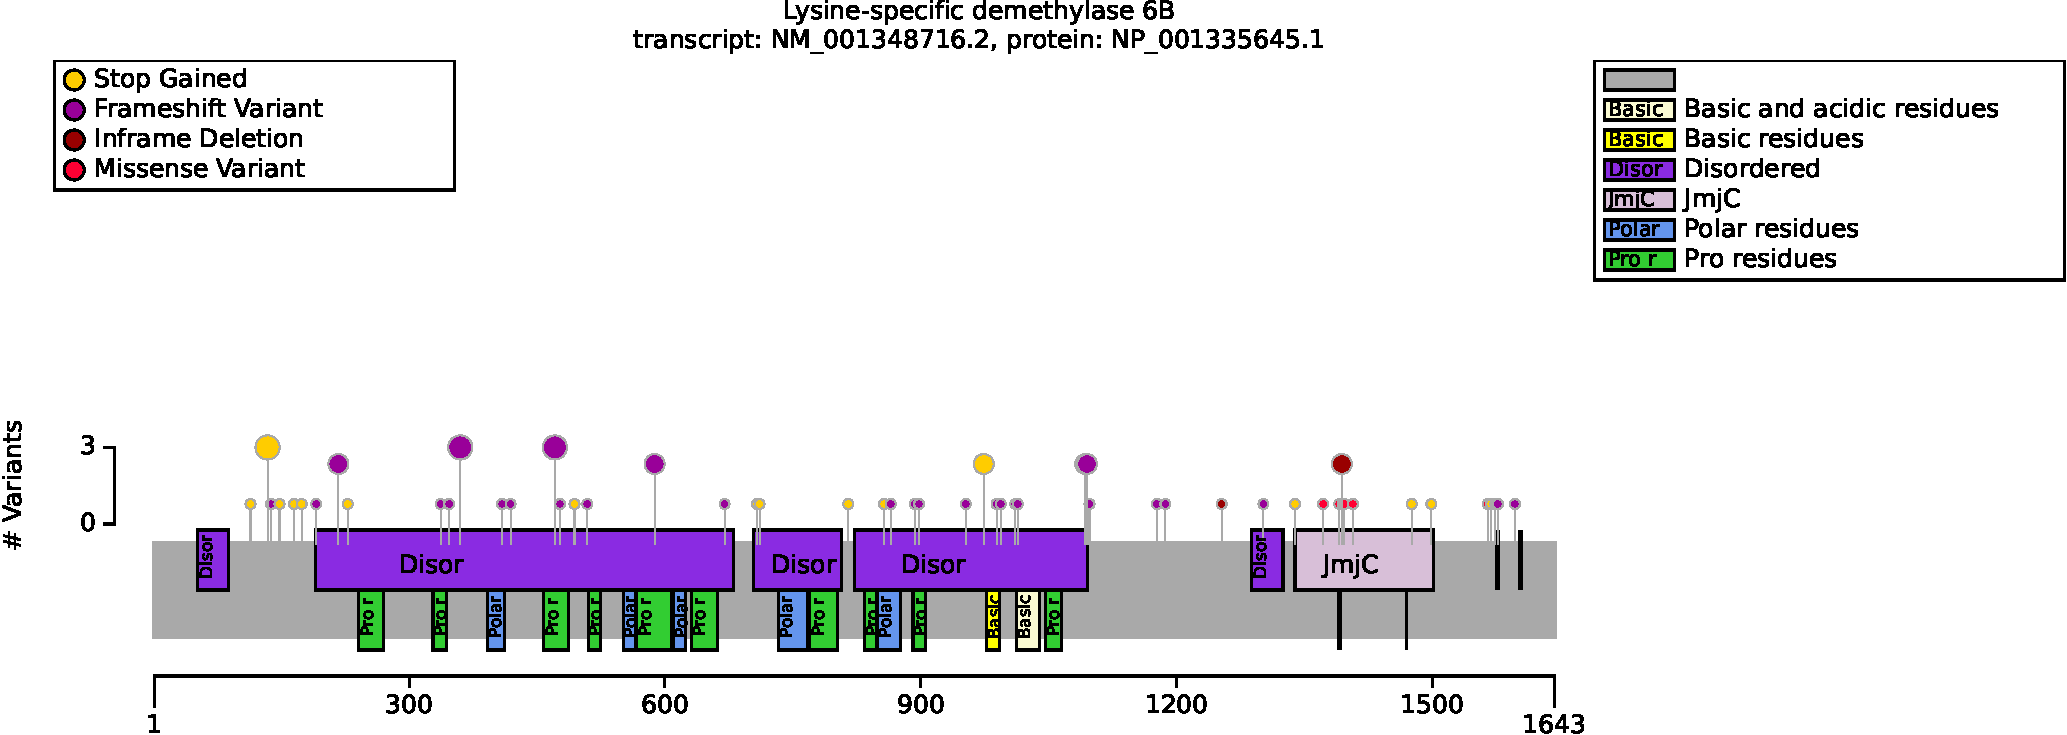
\includegraphics[width=\textwidth]{ img/KDM6B_protein_diagram.pdf} 
\captionsetup{justification=raggedright,singlelinecheck=false}
\caption{Distribution of variants in KDM6B}
\end{subfigure}

\vspace{2em}

\begin{subfigure}[b]{0.95\textwidth}
\centering
\resizebox{\textwidth}{!}{
\begin{tabular}{llllrr}
\toprule
Genotype (A) & Genotype (B) & total tests performed & significant results\\
\midrule
JmjC domain & Other & 54 & 0\\
N term & C term & 54 & 0\\
\bottomrule
\end{tabular}
}
\captionsetup{justification=raggedright,singlelinecheck=false}
\caption{Fisher Exact Test performed to compare HPO annotation frequency with respect to genotypes. }
\end{subfigure}

\vspace{2em}

\caption{The cohort comprised 73 individuals (19 females, 54 males). A total of 251 HPO terms were used to annotate the cohort. Disease diagnosis: Neurodevelopmental disorder with coarse facies and mild distal skeletal abnormalities (OMIM:618505). Stolerman et al (2016) identified no significant genotype-phenotype correlations \cite{PMID_31124279} A total of 61 unique variant alleles were found in \textit{KDM6B} (transcript: \texttt{NM\_001348716.2}, protein id: \texttt{NP\_001335645.1}).}
\end{figure}
